\documentclass[a4paper]{article}

\title{Documentation of the R package epiphylo}
\author{Xavier Didelot}

\usepackage{Sweave}
\begin{document}
\Sconcordance{concordance:epiphylo.tex:epiphylo.Rnw:%
1 5 1 1 0 4 1 1 5 1 1 1 2 4 0 1 2 3 1 1 2 5 0 1 2 3 1 1 2 1 0 3 1 4 0 1 %
2 3 1}

%\VignetteIndexEntry{Using epiphylo}

\maketitle


\section{Simulation}

A pathogen has an effective within-host population size of $N_e=100$ and a generation time $g=1$ day, so that $N_e g=100/365$ years. The basic reproduction number is $R=1$. To following command simulates an outbreak of this pathogen with 10 sampled cases: 
\begin{Schunk}
\begin{Sinput}
> simu <- simulateOutbreak(R=1,neg=100/365,ninf=10,pi=0.5)
\end{Sinput}
\end{Schunk}

This simulation contains both the transmission tree between infected hosts and the within-host phlogenetic tree of each host. This can be visualised as a colored phlogenetic tree, where each host is represented by a unique color:

\begin{center}
\begin{Schunk}
\begin{Sinput}
> plotBothTree(simu)
\end{Sinput}
\end{Schunk}
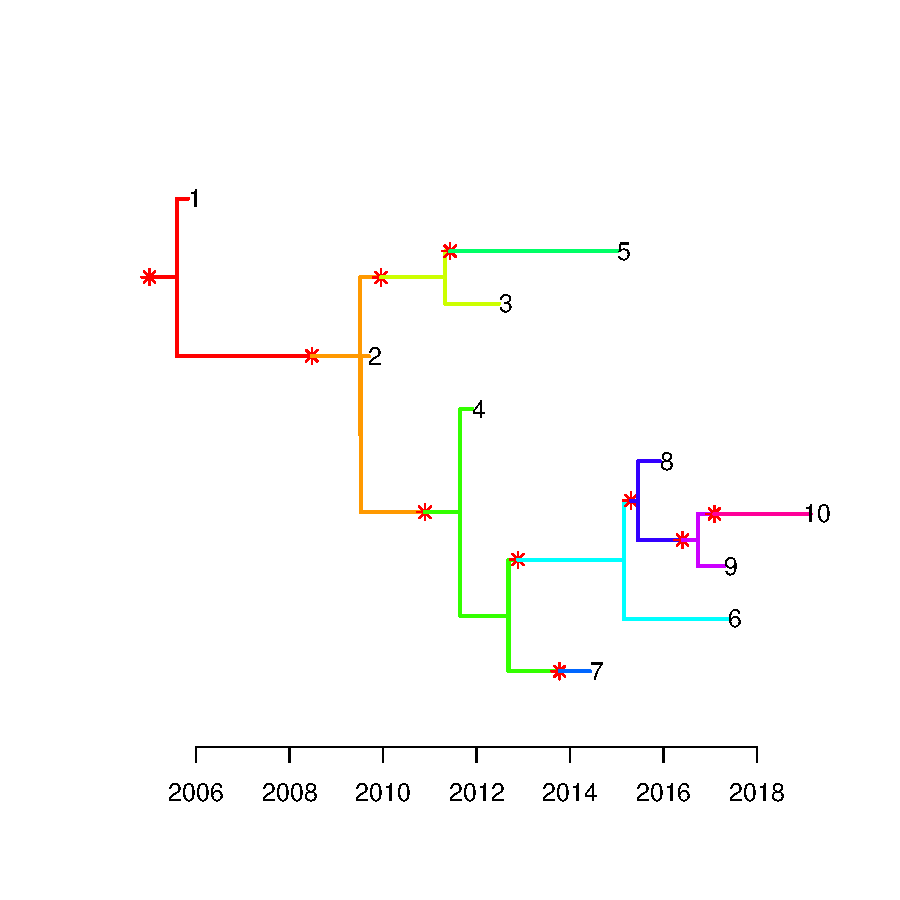
\includegraphics{epiphylo-003}
\end{center}

The transmission tree can be extracted and plotted separately from the phylogeny:

\begin{Schunk}
\begin{Sinput}
> ttree<-ttreeFromFullTree(simu)
> plotTTree(ttree)
\end{Sinput}
\end{Schunk}
\includegraphics{epiphylo-004}

The phylogenetic tree can be extracted and converted into a phylo object from the ape package:

\begin{Schunk}
\begin{Sinput}
> library(ape)
> ptree<-ptreeFromFullTree(simu)
> p<-phyloFromPtree(ptree)
> plot(p)
\end{Sinput}
\end{Schunk}
\includegraphics{epiphylo-005}

\section{Inference of transmission tree given a phylogeny}

A phylo object can be turned  into a phylogenetic tree and complemented with a wild guess at the transmission tree in order to provide the starting point of the MCMC procedure:

\begin{Schunk}
\begin{Sinput}
> ptree<-ptreeFromPhylo(p,dateLastSample=max(simu[,1]))
> full<-makeFullTreeFromPTree(ptree)
> plotBothTree(full)
\end{Sinput}
\end{Schunk}
\includegraphics{epiphylo-006}

The MCMC procedure to infer the transmission tree given the phylogenetic tree can be run as follows:

\begin{Schunk}
\begin{Sinput}
> record<-inferTTree(ptree,mcmcIterations=100)
\end{Sinput}
\end{Schunk}

This returns a record of all MCMC iterations. This is what the transmission tree looks like at the end of the MCMC:

\begin{Schunk}
\begin{Sinput}
> lastIteration<-record[[length(record)]]
> plotBothTree(lastIteration$tree)
\end{Sinput}
\end{Schunk}
\includegraphics{epiphylo-008}

Traces of the MCMC:

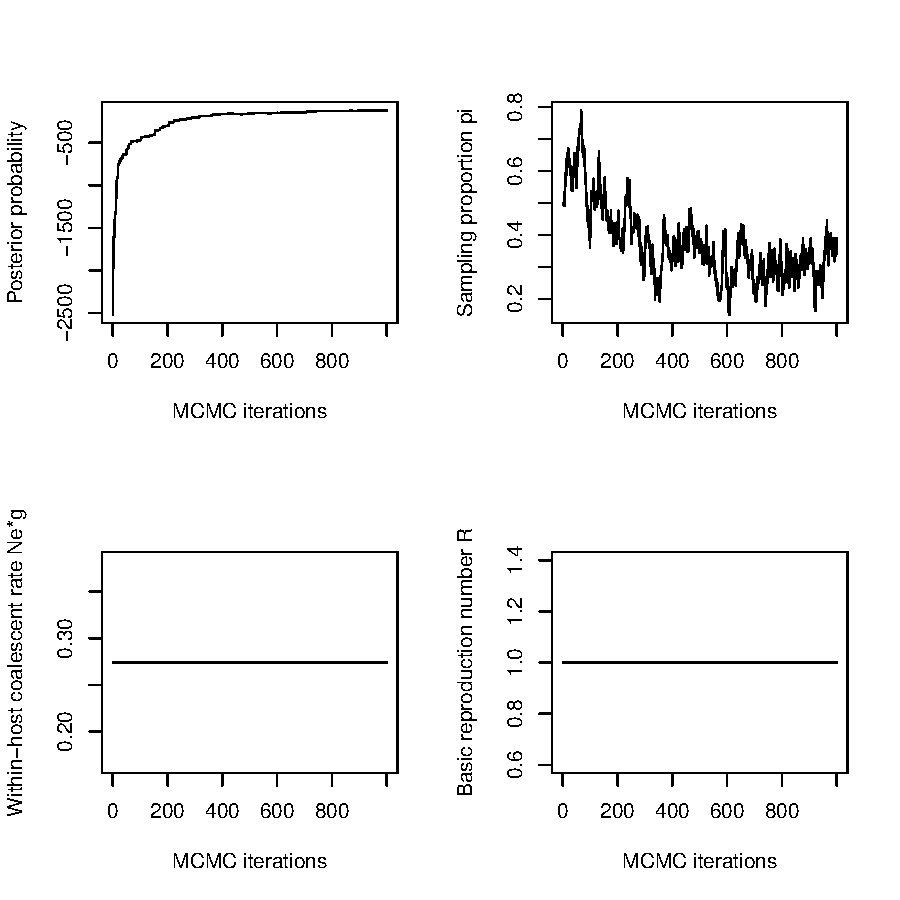
\includegraphics{epiphylo-009}

\end{document}
